\documentclass[a4paper,titlepage,twoside,12pt,leqno]{article}

\usepackage[]{fontspec}
\usepackage{xltxtra}
\usepackage[monogreek]{xgreek}

\newcommand{\en}[1]{\setlanguage{american}#1\setlanguage{monogreek}} % Για υφενώσεις στα αγγλικά

\defaultfontfeatures{Mapping=tex-text%, Scale=MatchLowercase}
} 

% Γραμματοσειρά
\setmainfont[Mapping=tex-text]{DejaVu Sans}


\usepackage{longtable} % για έναν μεγάλο πίνακα
\usepackage{graphicx, array, blindtext}

\title{Αναλυτικό εγχειρίδιο αναφοράς για το ηλεκτρονικό θεματικό πάρκο σε μεσαιωνική καστροπολιτεία}
\author{Αναγνωστόπουλος Βασίλης-Θάνος, Κατσής Γιώργος}
\date{}

\begin{document}

\maketitle
\tableofcontents
\listoffigures
\listoftables
\newpage

\section{Εισαγωγή}

%Στα εγχειρίδια αυτά παρουσιάζεται η σύνταξη όλων των εντολών του προγράμματος. Σε αυτά τα εγχειρίδια ανατρέχει ένας χρήστης για να βρει την σύνταξη της οποιασδήποτε εντολής. Ο στόχος των εγχειριδίων αυτών είναι να καλύψουν πλήρως τη λειτουργία ενός προγράμματος και όχι να εκπαιδεύσουν το χρήστη. Αυτά τα εγχειρίδια χρησιμεύουν σε όλους τους χρήστες, είτε αυτοί είναι καινούριοι είτε παλαιότεροι οπότε γνωρίζουν λίγο πολύ τη λειτουργία του προγράμματος.

%\emph{Σημείωση: Τα κείμενα το οποία είναι γραμμένα σε πλάγια γραφή (όπως και το συγκεκριμένο) είναι σημειώσεις, οι οποίες θα απομακρυνθούν από το τελικό κείμενο, αλλά αυτή την στιγμή υποδηλώνουν εργασίες οι οποίες δεν μπορούν να ολοκληρωθούν χωρίς να αναπτυχθεί ο κώδικας της εφαρμογής ή για κάποιο άλλο παρεμφερή λόγο.\\}

Σε αυτό το κείμενο αναλύονται οι δυνατότητες του προγράμματος που υπάρχει στους υπολογιστές της καστροπολιτείας.

Το συγκεκριμένο πρόγραμμα προορίζεται για την αλληλεπίδραση των ενοίκων του μεσαιωνικού καστροδιαμερίσματος με τις διάφορες συσκευές και υπηρεσίες που διαθέτει το διαμέρισμα του και η καστροπολιτεία. Συνοπτικά μέσα αυτού του προγράμματος μπορείτε να πραγματοποιήσετε τα παρακάτω:

\begin{itemize}
\item έλεγχο των συσκευών του διαμερίσματος σας όπως η πόρτα του διαμερίσματος του, το ραδιόφωνο κ.λ.π. (βλέπε σελ. \ref{syskeuves})
\item τον έλεγχο της θερμοκρασίας και της στάθμης της πισίνα καθώς και απενεργοποίηση του συναγερμού της πισίνας. (βλέπε σελ. \ref{pisina})
\item να πραγματοποιήσετε παραγγελίες στο εστιατόριο της καστροπολιτείας (βλ. σελ. \ref{paraggelia}).
\end{itemize}

%\emph{Σημείωση: Εδώ θα μπει η πλήρης λίστα με τις συσκευές που μπορεί να αλληλεπιδράσει ο χρήστης καθώς και που βρίσκονται.}

\section{Πλοήγηση στην εφαρμογή}

%\emph{Σημείωση: Τα εγχειρίδια προτιμήθηκε να γραφούν σε λιγότερη επίσημη γλώσσα. Η επιλογή αυτή είναι λάθος; Επίσης τί κεφάλαια να περιλαμβάνονται σε αυτό το εγχειρίδιο;\\}

Η πρώτη οθόνη της εφαρμογής είναι για την επιλογή του κατάλληλου μενού για την αλληλεπίδραση με την καστροπολιτεία. Στα δεξιά του παραθύρου φαίνονται σημαίες από χώρες και πατώντας κάποια σημαία αλλάζει η γλώσσα των μηνυμάτων που εμφανίζονται στην εφαρμογή.

Στα αριστερά της εφαρμογής φαίνονται τα εικονίδια επιλογών καθώς και ένα μικρό κείμενο το οποίο επεξηγεί τί κάνει το καθένα (βλ. σχήμα \ref{fig:menu:general})

\begin{figure}
\begin{center}
\resizebox*{\textwidth}{!}{
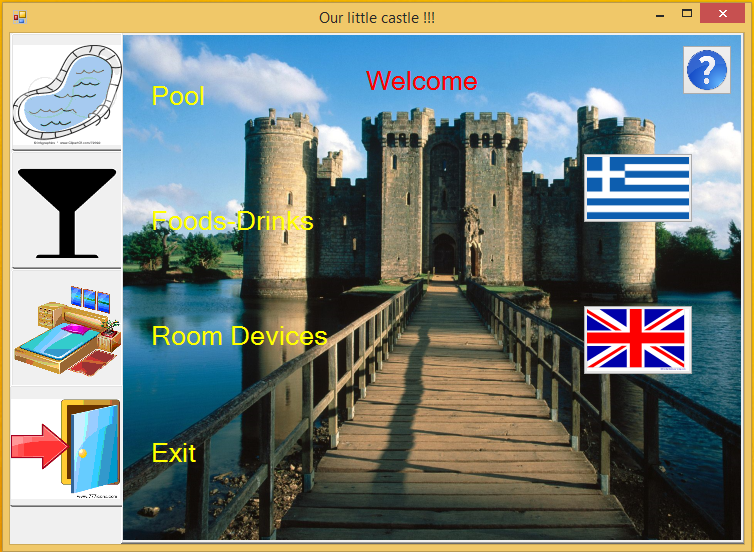
\includegraphics{images/ScreenExit.png}}
\caption{Το εισαγωγικό μενού.}
\label{fig:menu:general}
\end{center}
\end{figure}

Στον πίνακα \ref{table:icons} φαίνονται αναλυτικά τα εικονίδια καθώς και το τί κάνουν.

\begin{table}
\begin{center}
  \begin{tabular}{|m{0.20\textwidth}|m{0.70\textwidth}|}
    \hline
     
     \vspace{0.3cm}
     \resizebox*{0.20\textwidth}{!}{
     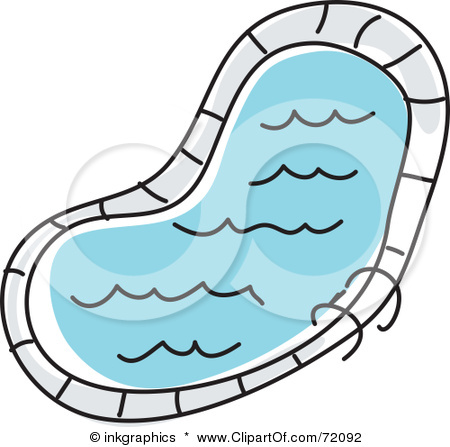
\includegraphics{images/pool.jpg}}

     & Πατώντας το συγκεκριμένο εικονίδιο μεταβαίνουμε στο μενού για τον έλεγχο της πισίνας. \\ \hline

     \vspace{0.3cm}
     \resizebox*{0.20\textwidth}{!}{
     
\includegraphics{images/glass.png}}

     & Πατώντας το συγκεκριμένο εικονίδιο μεταβαίνουμε στο μενού των παραγγελιών. \\ \hline

     \vspace{0.3cm}
     \resizebox*{0.20\textwidth}{!}{
     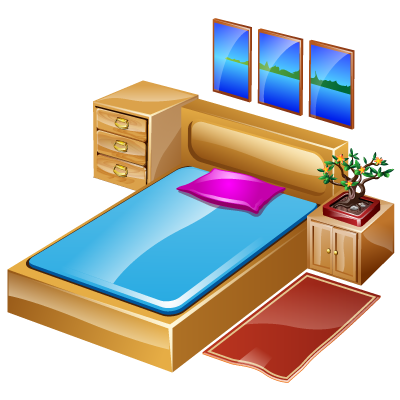
\includegraphics{images/bedroom.png}}

     & Πατώντας το συγκεκριμένο εικονίδιο μεταβαίνουμε στο μενού ελέγχου των συσκευών του δωματίου. \\ \hline

     \vspace{0.3cm}
     \resizebox*{0.20\textwidth}{!}{
     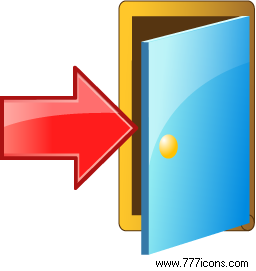
\includegraphics{images/exit.png}}

     & Πατώντας το συγκεκριμένο εικονίδιο μεταβαίνουμε στην αρχική οθόνη. \\ \hline
  \end{tabular}
\caption{Τα εικονίδια της εφαρμογής}
\label{table:icons}
\end{center}
\end{table}

%\emph{\\Σημείωση: Εδώ θα μπει πίνακας για να τα επεξηγεί, αλλά από την στιγμή που δεν έχει αποφασιστεί ακόμα το σχήμα τους και η λειτουργικότητα τους παραλείφθηκαν.\\}

Όταν πατηθεί κάποιο εικονίδιο τότε γίνεται μετάβαση σε ένα νέο παράθυρο το οποίο αλλάζει ανάλογα με την επιλογή, όμως το μενού με τα εικονίδια στα αριστερά παραμένει έτσι ώστε να είναι δυνατή η εναλλαγή μεταξύ των μενού γρήγορα χωρίς ο χρήστης να είναι υποχρεωμένος να γυρίσει στην αρχική οθόνη.

\section{Παραγγελία αντικειμένων}
\label{paraggelia}

Σε αυτό το μενού μπορούμε να παραγγείλουμε προϊόντα από την καφετέρια-εστιατόριο της καστροπολιτείας μας. Για να εισέλθουμε σε αυτό το μενού θα πρέπει να πατήσουμε το εικονίδιο που μοιάζει με ποτήρι από το κεντρικό μενού (βλ. σχήμα \ref{fig:icon:order}).

%\emph{\\Σημείωση: Επειδή ακόμα δεν έχουν αποσαφηνιστεί η λεπτομέρειες με τα εικονίδια αφέθηκαν κενά.\\}
\begin{figure}
\begin{center}
\resizebox*{0.20\textwidth}{!}{

\includegraphics{images/glass.png}}
\caption{Το εικονίδιο για να μεταβούμε στο μενού των παραγγελιών.}
\label{fig:icon:order}
\end{center}
\end{figure}

Στα αριστερά του μενού μπορεί ο χρήστης να διαλέξει ανάμεσα σε φαγητό ή ποτό και εμφανίζεται η κατάλληλη καρτέλα με τις επιλογές του χρήστη. (βλ. σχήμα \ref{fig:menu:order-food} και \ref{fig:menu:order-drinks}).

Ο χρήστης μετά μπορεί να επιλέξει όποιο προϊόν επιθυμεί και για να ολοκληρώσει την παραγγελία του θα πρέπει να πατήσει το κουμπί της πληρωμής. Μόλις το πατήσει θα εμφανιστούν κατάλληλα μηνύματα που θα τον καθοδηγούν για την πληρωμή της παραγγελίας τους (βλ. σχήμα \ref{fig:menu:order-payment}). Εναλλακτικά μπορεί να πατήσει ακύρωση για την ακύρωση της παραγγελίας του.

\begin{figure}
\begin{center}
\resizebox*{\textwidth}{!}{
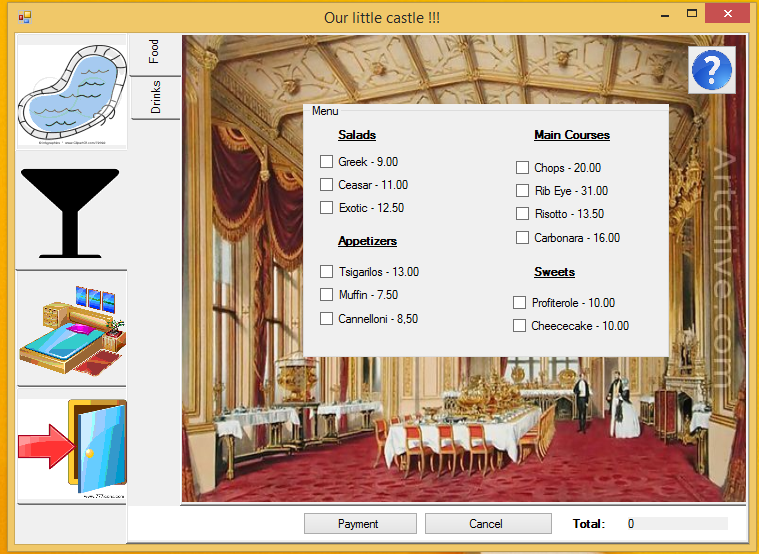
\includegraphics{images/SreenFood.png}}
\caption{Το μενού των παραγγελιών.}
\label{fig:menu:order-food}
\end{center}
\end{figure}

\begin{figure}
\begin{center}
\resizebox*{\textwidth}{!}{
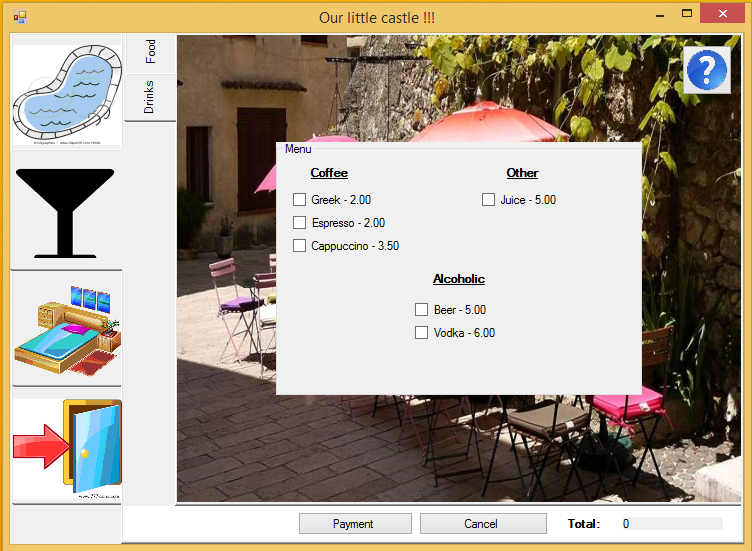
\includegraphics{images/ScreenDrinks.png}}
\caption{Το μενού των παραγγελιών (2).}
\label{fig:menu:order-drinks}
\end{center}
\end{figure}

\begin{figure}
\begin{center}
\resizebox*{0.75\textwidth}{!}{
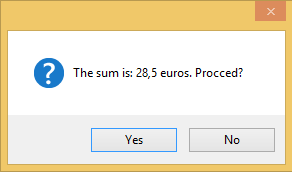
\includegraphics{images/MessagePayment.png}}
\caption{Η ολοκλήρωση της παραγγελίας.}
\label{fig:menu:order-payment}
\end{center}
\end{figure}

\newpage

\section{Διαχείριση τάφρου-πισίνας}
\label{pisina}

Σε αυτό το μενού μπορούμε να διαχειριστούμε την πισίνα-τάφρο του διαμερίσματος. Για να εισέλθουμε σε αυτό το μενού θα πρέπει να πατήσουμε το εικονίδιο που μοιάζει με πισίνα (βλ. σχήμα \ref{fig:icon:pool}) από το κεντρικό μενού (βλ. σχήμα \ref{fig:menu:pool}).

\begin{figure}
\begin{center}
\resizebox*{0.20\textwidth}{!}{
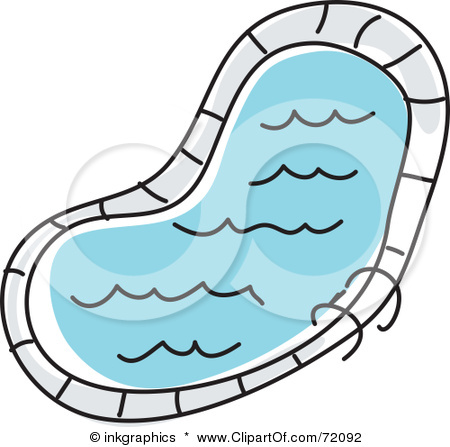
\includegraphics{images/pool.jpg}}
\caption{Το εικονίδιο για να μεταβούμε στο μενού των παραγγελιών.}
\label{fig:icon:pool}
\end{center}
\end{figure}

\begin{figure}
\begin{center}
\resizebox*{\textwidth}{!}{
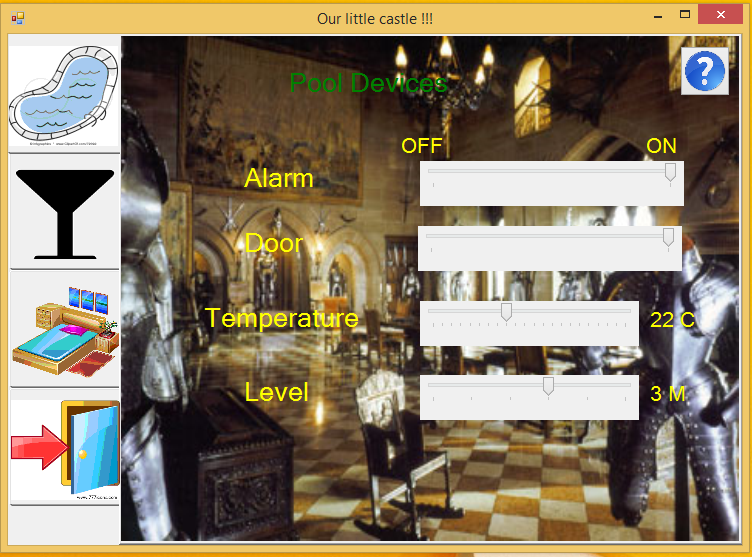
\includegraphics{images/ScreenPool.png}}
\caption{Το μενού χειρισμού της πισίνας του διαμερίσματος.}
\label{fig:menu:pool}
\end{center}
\end{figure}

Από αυτό το μενού ο χρήστης μπορεί να ρυθμίσει όλες τις πτυχές της πισίνας του διαμερίσματος. Συγκεκριμένα μπορεί να ενεργοποιηθεί ο συναγερμός που ελέγχει αν υπάρχουν άνθρωποι μέσα στην πισίνα (από την πρώτη μπάρα του συγκεκριμένου μενού), να ανοίξει/κλείσει η πόρτα της πισίνας (από την δεύτερη μπάρα), η θερμοκρασία και η στάθμη της πισίνας (από την 3η και 4η μπάρα αντίστοιχα)

Οι δύο πρώτες μπάρες ενεργοποιούν τον συναγερμό και ανοίγουν την πόρτα αντίστοιχα σέρνωντας τημ μπάρα προς τα δεξιά ενώ απενεργοποιούν τον συναγερμό και κλείνουν την πόρτα αντίστοιχα σέρνωντας την μπάρα προς τα αριστερα.

Ομοίως και οι δύο τελευταίες μπάρες σέρνωντας τες προς τα δεξία αυξάνεται η θερμοκρασία/ στάθμη και σέρνωντας της προς τα αριστέρα μειώνεται η θερμοκρασία/στάθμη.

%\emph{\\Σημείωση: Επειδή ακόμα δεν έχουν υλοποιηθεί εδώ φαίνεται μόνο πως θα είναι στο περίπου το εγχειρίδιο. Όταν υλοποιηθεί η εφαρμογή θα συμπληρωθούν και τα υπόλοιπα. Ομοίως θα είναι και τα υπόλοιπα κεφάλαια αλλά ακόμα δεν έχουν συμπληρωθεί.\\}




\newpage

\section{Διαχείριση ηλεκτρονικών συσκευών}
\label{syskeuves}

Από αυτό το μενού μπορούμε να διαχειριστούμε την διάφορες συσκευές που υπάρχουν μέσα στο διαμέρισμα. Για να εισέλθουμε σε αυτό το μενού θα πρέπει να πατήσουμε το εικονίδιο που μοιάζει με κρεβάτι (βλ. σχήμα \ref{fig:icon:room}) από το κεντρικό μενού (βλ. σχήμα \ref{fig:menu:room}).

\begin{figure}
\begin{center}
\resizebox*{0.20\textwidth}{!}{
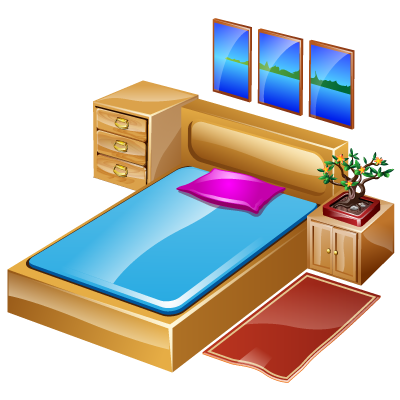
\includegraphics{images/bedroom.png}}
\caption{Το εικονίδιο για να μεταβούμε στη διαχείρηση των ηλεκτρικών συσκευών.}
\label{fig:icon:room}
\end{center}
\end{figure}

\begin{figure}
\begin{center}
\resizebox*{\textwidth}{!}{
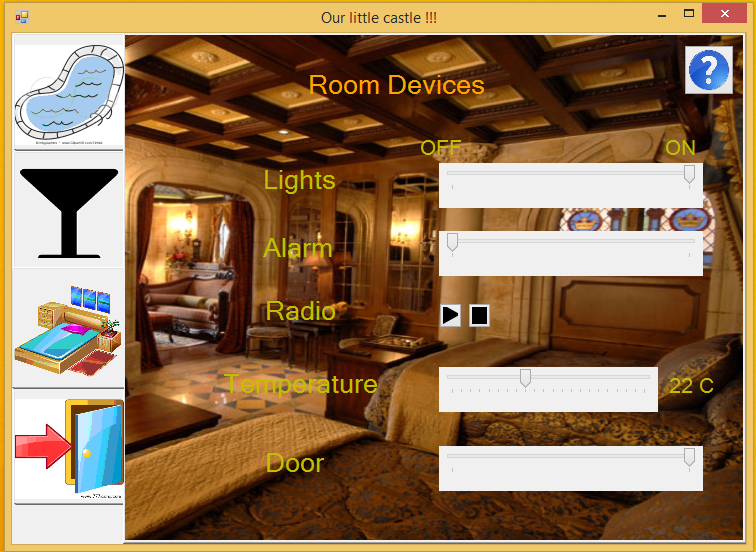
\includegraphics{images/SreenRoom.png}}
\caption{Το μενού χειρισμού των συσκεών των ηλεκτρονικών συσκευών.}
\label{fig:menu:room}
\end{center}
\end{figure}

Από αυτό το μενού ο χρήστης μπορεί να ρυθμίσει όλες τις συσκεύες που υπάρχουν μέσα στο δωμάτιο του στην καστροπολιτεία. Συγκεκριμένα μπορεί να ενεργοποιήσει/απενεργοποιήσει τα φώτα (από των πρώτη μπάρα), τον συναγερμό του δωματίου του (από την δεύτερη μπάρα), να ενεργοποιήσει/απενεργοποιήσει το ραδιόφωνο, να ανοίξει/κλείσει την πόρτα (από την τελευταία μπάρα) και να ρυθμίσει την θερμοκρασία του δωματίου (από την προ-τελευταία μπαρα).

Συγκεκριμένα σέρνωντας την μπάρα προς τα δεξία ενεργοποιείται η αντίστοιχη συσκευή ενώ σέρνωντας την προς τα αριστερά απενεργοποιείται.


%\emph{\\Σημείωση: Τί άλλα κεφάλαια να βάλουμε σε αυτό το εγχειρίδιο και γενικά ποια να είναι η δομή του.\\}


\end{document}
